\documentclass[../main-v1.tex]{subfiles}
\begin{document}
\chapter{Data Management \hideme{Timm, Mandrichenko - draft} }
\label{ch:datamgmt}

%%%%%%%%%%%%%%%%%%%%%%%%%%%%%%%%
\section{Introduction \hideme{HMS update 3/9}}
\label{sec:datamgmt:xyz}  %% fix label according to section

The Data Management subsystem brings data from the detectors to the archival storage facility 
and then distributes it to storage elements around the world.  The components include a data ingest manager, a replica manager that knows the location of files and manages the transfers between storage elements, a metadata catalog that keeps track of the types and provenance of data, and an interface to deliver the appropriate files to the workflow management system and interactive users.

The DUNE Data Management group is currently designing and deploying several new components in the Data Management
system, to replace the legacy \dword{sam}~\cite{Illingworth:2014mba} system, which combined the functions of replica manager, metadata server, 
and file delivery.  Those functions are being separated with well defined interfaces.  The goal is to have the new systems in place before beam running begins on \dword{pdsp2}. %pdhd}.
%Kirby changed \dword{pdsp2} %HMS - is this ok now? anne ProtoDUNE-II (single-phase ) (horizontal drift).  

Figures \ref{fig:datamanagement_old} and \ref{fig:datamanagement} illustrate the old and proposed data management architectures with the legacy \dword{sam} system replaced by a new catalog and the \dword{rucio} storage management systems. 

%\todo{Put a figure showing current and future architectures here}
\begin{dunefigure}
[SAM Data management architecture diagram]
{fig:datamanagement_old} 
{Legacy \dword{sam} data management architecture.  The \dword{sam} system provides both catalog and data location information to processing nodes.}
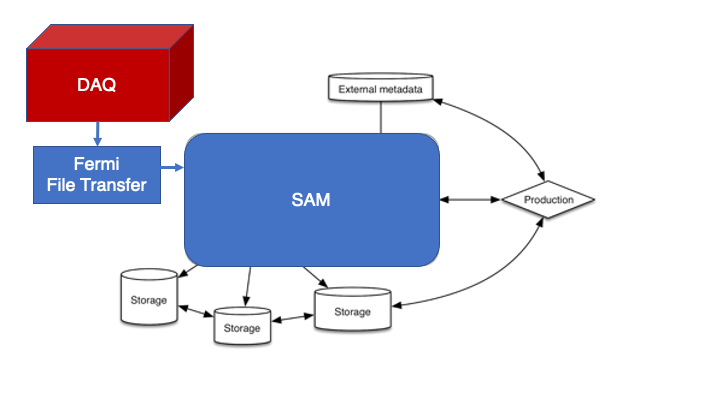
\includegraphics[height=8cm]{graphics/DataManagement/data_mgmt_figures_old.png}
\end{dunefigure}

\begin{dunefigure}
[New Data management architecture diagram]
{fig:datamanagement} 
{Proposed data management architecture diagram.  The \dword{sam} functions are divided between the \dword{metacat} catalog, the \dword{rucio} data movement system and a \dword{datadis} that interfaces to processing and monitoring systems.  }
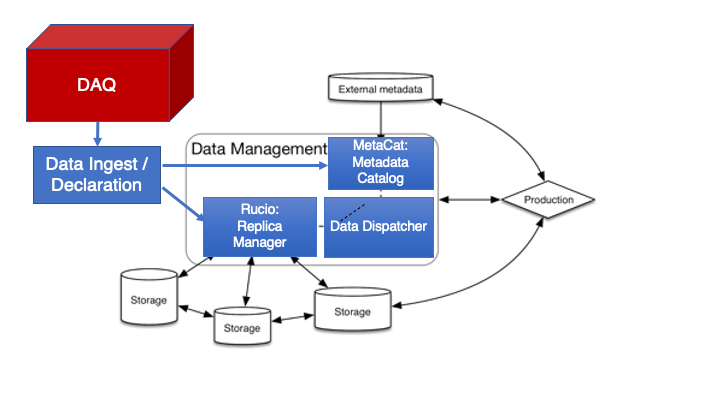
\includegraphics[height=8cm]{graphics/DataManagement/data_mgmt_figures.png}
\end{dunefigure}
%\todo{Get better figure}

%\todo{Need to insert basic data management architecture here}

%\label{ch:sam:catalog}

%\hideme{Decide what to do with the catalog section}
%\section{Existing SAM Data Management System}

The existing DUNE data catalog, \dword{sam}, was originally designed for the D0 and CDF high energy physics experiments at \dword{fnal}.  It is now used by most of the Intensity Frontier experiments at Fermilab. %HMS DONE 3/9 anne Fermilab. 

The most important objects cataloged in \dword{sam} are individual files and collections of files called
\dwords{samdataset}.
Data files themselves are not stored in \dword{sam}, their metadata is, and that metadata allows users to both identify and locate the physical files %HMS DONE 3/9 anne you to searc and find 
%searching for the actual physical files.

%anne can't have one subsection under a section; need at least two \subsection{General considerations}

\dword{sam} was designed to ensure that large-scale data processing be done accurately and completely,  which led to  high standards of reproducibility and documentation in data analysis.
For example, at the time of the original design, the main storage medium was 8\,mm tapes using consumer-grade drives.  Drive and tape failure rates were $>1$\%.  Several \dword{sam} design concepts, notably luminosity blocks and parentage tracking, were introduced to allow accurate tracking of files and their associated normalization in a high error-rate environment. 

\dword{sam} is almost completely file-based and duplicates run-level information.  The %\dword{sam} 
system has seen us through the first \dword{protodune} runs but going forward, a replacement is needed. %HMS OK anne moved to above req section

\section{Requirements for Replacing SAM Functionality \hideme{HMS update 3/9}}


% Goals of \dword{sam} replacement : Generalized from events and files to objects and collections

% Collections could be long trigger records, data from different detectors over a particular time period, …

 The replacement for \dword{sam} should support use of run or trigger record level information, in addition to file information,  as appropriate. 
For example,  DUNE trigger records may span multiple files. The new model needs to generalize from ``events'' and files to data objects and collections across multiple scales. 

%Here we list the existing 
The functions of the existing \dword{sam} system that we wish to retain and extend are listed here. The first three functions %anne goals 
relate to content and characteristics while the last four relate to data storage and processing tools.  We propose to separate these functions where appropriate.

\begin{enumerate}

\item	Describe the contents of individual files in a searchable manner. 

\item	Create and document data collections ``datasets'' to allow later retrieval based on data characteristics.

 \item	Track object and collection parentage and describe processing transformations to document the full provenance of any data object and ensure accurate normalization.

 %\item	Group  objects and collection into larger “datasets” based on their characteristics

 \item	Store the physical  location of objects.

 \item	Track the processing of collections to allow reprocessing on failure and avoid double processing.

 \item	Provide methods for delivering and tracking collections in multi-process jobs.

 \item	Preserve data about processing/storage operations for debugging/reporting.

\end{enumerate}
 We propose to break the existing system up into functional sub-units specializing in cataloging, storage and delivery. 

\begin{description}
\item{\bf \dshort{metacat}}  The catalog function will be replaced by a combination of a file metadata catalog \dword{metacat} and a run configuration database that stores run level information.
\item{\bf \dshort{rucio}}  The file location function is replaced by \dword{rucio}~\cite{Barisits:2019fyl}, the file tracking system originally developed by the ATLAS collaboration. \dword{rucio} provides a location catalog for files and rule-based transfers between sites. 
%\todo{(anne) Can we adjust the dword def of samproject to include SAM? Just 'project' is too general. HMS done for project but other consepts remain in new version os can't just say sam.}
\item{\bf Data Dispatcher} The existing \dword{sam} system supports a station and \dword{samproject} ecosystem where \dwords{samdataset} are submitted for processing as \dwords{samproject}.  The \dword{samproject} is a server process that contains a list of files based on a \dword{samdataset} description  and, when asked, delivers location information for the next file in the list.  Request, delivery and processing are tracked and recorded. This allows resubmission on failure. A website allows users to see the details of file delivery. 
%\item{\bf \dshort{fts}} \todo{(anne) missing content - HMS 3/9 decide to move elsewhere as this woudl be describibg an existing service parallel to but not part of sam}


\end{description}



% \begin{enumerate}

% \item 	The current \dword{sam} implementation uses the file as the basic unit of information.  Metadata is associated with the file name.  Filenames much be unique in the system. This prevents duplication of data in a sample, as a second copy cannot be cataloged. %This makes renaming a file very unwise. A very common practice is to include some of the metadata in the filename, both to make it easier to identify and to ensure uniqueness.    

% A \dword{sam} replacement needs to move away from physical files as the unit of data collection.  Data collections should be hierarchical with collections able to contain other collections.

% Metadata can be associated with an object, a time period (runs), a processing step or a configuration (runs). Objects/data collections need pointers to the appropriate configuration. 

% \item	Metadata for a file can include file locations but does not have to. A file can have no location at all, or many. When you move or remove a file with an associated \dword{sam} location, you need to update the location information.
% Rucio will handle this location but mapping to data collections needs to be clear and robust. 

 

% \item	Files which are stored on disk or tape are expected to have appropriate file sizes and checksums. One can have duplicate instances of a file in different locations, but they must all be identical.  


% \item	Files can have parents and children and, effectively birth certificates that can tell you how they were made.  An example would be a set of raw data files RAWnnn processed with code X to produce a single reconstructed file RECO.  One can tell \dword{sam} that RAWnnn are the parents of RECO processed with version x of code X. If one later finds another RAWnnn file that was missed in processing, \dword{sam} can tell you it has not been processed yet with X (i.e., it has no children associated with version x of X) and you can then choose to process that file. This use case often occurs when a production job fails without reporting back or succeeds but the copy back or catalog action fails. 

% This provenance information is important to retain at the object and collection level. 

% The D0 experiment required that all official processing going into \dword{sam} be done with tagged releases and fixed parameter sets to increase reproducibility and the tags for that information were included in the metadata. Calibration databases were harder to timestamp so some variability was still possible if calibrations were updated.

In the following subsections we describe the existing features in more detail with the proposed replacement technologies in %following 
later sections. 

\subsection{Existing SAM  Features}

\subsubsection{Data Description Values and Parameters}

 \dword{sam} supports several types of data description fields.
% Values are common across all implementations and optimized for fast retrieval.  High level concepts such as data tier and detector type are example. 
% Parameters are defined by the experiment and are extensible.
\dword{sam}  Generic ``values'' such as data\_tier, run\_type and file\_size  are common to almost all  HEP experiments and are optimized for efficient queries.  \dword{sam} also allows definition of free-form ``parameters'' as they are needed within each experiment's instance.  This allows the schema to be modified easily as needs arise.  \dword{metacat} extends these concepts to make them easier to search and maintain. 

% a.	We need optimized types for those most frequently used

% b.	We need expandable but enumerated types for important types.  Example would be detector configurations, which need to be added per experiment but should have a small set of valid values and not allow free form entries. 

% c.	We also need free form entries to annotate objects and collections. 

% Currently \dword{sam} values cover case a. and parameters cover case c. but it is not possible to list all possible values for a parameter without looping over all files. 

% 8.  Metadata can also contain “spill” or luminosity block information that allows a file to point to specific data taking periods with smaller granularity than a run or subrun. When files are merged, this spill information is also merged.

In the following %anne example file metadata
sample metadata file from DUNE, generic \dword{sam} values are listed first followed by experiment specific parameters. The items starting with beam.momentum or containing ``.'' in their names are parameters. Many of the parameter entries are specific to the run configuration, not the individual file, and will move in the new design. \fixme{will move to a different type of file? pls clarify "move" here (anne)}

\begin{verbatim}

{
 "file_name": "np04_raw_run005141_0015_dl10_reco_12736632_0_20181028T182951.root", 
 "file_id": 7352771, 
 "create_date": "2018-10-29T14:59:42+00:00", 
 "user": "dunepro", 
 "update_date": "2018-11-28T17:07:30+00:00", 
 "update_user": "schellma", 
 "file_size": 14264091111, 
 "checksum": [
  "enstore:1390300706", 
  "adler32:e8bf4e23"
 ], 
 "content_status": "good", 
 "file_type": "detector", 
 "file_format": "artroot", 
 "data_tier": "full-reconstructed", 
 "application": {
  "family": "art", 
  "name": "reco", 
  "version": "v07_08_00_03"
 }, 
 "event_count": 108, 
 "first_event": 21391, 
 "last_event": 22802, 
 "start_time": "2018-10-28T17:34:58+00:00", 
 "end_time": "2018-10-29T14:55:42+00:00", 
 "data_stream": "physics", 
 "runs": [
  [
   5141, 
   1, 
   "protodune-sp"
  ]
 ], 
 "parents": [
  {
   "file_name": "np04_raw_run005141_0015_dl10.root", 
   "file_id": 6607417
  }
 ],
 "beam.momentum": 7.0, 
 "data_quality.online_good_run_list": 1, 
 "detector.hv_value": 180, 
 "DUNE_data.acCouple": 0, 
 "DUNE_data.calibpulsemode": 0, 
 "DUNE_data.DAQConfigName": "np04_WibsReal_Ssps_BeamTrig_00021", 
 "DUNE_data.detector_config": "cob2_rce01:.. 4 more lines of text", 
 "DUNE_data.feshapingtime": 2, 
 "DUNE_data.inconsistent_hw_config": 0, 
 "DUNE_data.is_fake_data": 0, 
}



\end{verbatim}



\subsubsection{Event Catalog - Absence of}
\dword{sam} currently does not contain a means of easily determining which file(s) contains a given event.  If a \dword{daq} system is writing multiple streams, an event from a given subrun could be in any stream.   Existing neutrino experiments are low enough rate that this has not been an issue but \dword{protodune} already needs this feature.
The \dword{sam} replacement will require the development of a true two-way map between objects (events) and collections. 
\fixme{(anne) I'd move this above 'existing SAM features, because it's NOT one!}
 
% All of these features are intended to assure that your data are well described and can be found. As \dword{sam} stores full location information, this means any sam-visible location. In addition, if parentage information is provided, you can determine and reproduce the full provenance of any file.


\subsection{SAM Datasets and Projects}

\subsubsection{Datasets and Snapshots}

In addition to the files themselves, \dword{sam} allows %anne you to define
definition of \dwords{samdataset}.
%I think that somebody did this. I suspect Heidi? \todo{(anne) Can we adjust the dword defs of samdataset and samsnapshot (and others that might pop up) to include SAM?}
A  \dword{samdataset} is not a fixed list of files but a query against the \dword{sam} database. An example query would be ``data\_tier reconstructed and run\_number 2001 and version v10'' which would be all files from run 2001 that are reconstructed data produced by version v10. The \dword{samdataset} is dynamic; if after processing run 2001, an additional file from run 2001 is found
%Kirby - tried to clarify Mar 14, 2022 \todo{(anne) if one finds that a file that should be there is not there? Or if one finds a file that had been missing (and is now found)? Pls clarify}
and this additional file is reconstructed with v10, the \dword{samdataset} will grow to include it. There are also %\dword{samdataset} 
``\dwords{samsnapshot}'' that are derived from \dwords{samdataset} and capture the exact files in the \dword{samdataset} when the \dword{samsnapshot} was made.
%Note: most other data catalogs assume a “\dword{dataset}” is a fixed list of files.  This is a “snapshot” in sam. 

%Do we need to keep the mutable query or stick to defined versioned collections? 


% Samweb – samweb is the command line and python API that allows queries of the \dword{sam} metadata, creation of \dword{dataset}s and tools to track and deliver information to batch jobs.

% Will need an updated API

\subsubsection{SAM Projects}

%This is likely out of scope for the metadata themselves. 

\dword{sam} also supports access delivery and  tracking mechanisms called \dwords{samproject} and \dwords{samconsumer}.

A \dword{samproject} is effectively a processing campaign across a \dword{samdataset} that is owned by the \dword{sam} system. At launch, a snapshot is generated after which the files in the snapshot are delivered to a set of \dwords{samconsumer}.  The \dword{samproject} maintains an internal record of the status of the files and \dwords{samconsumer}. Compute processes instantiate \dwords{samconsumer} attached to the \dword{samproject}.  Those \dwords{samconsumer} then request ``files'' from the \dword{samproject} and, when done processing, tell the \dword{samproject} of their status.  

The original \dword{sam} implementation actually delivered the files to local hard drives.  Modern \dword{sam} delivers the location information and expects the \dword{samconsumer} to find the optimal delivery method. This is a pull model, where the consuming process requests the next file rather than having the file assigned to it.  This makes the system more robust on distributed systems. 
There is also a web interface\footnote{\href{http://samweb.fnal.gov:8480/station_monitor/dune/stations/dune/projects}{http://samweb.fnal.gov:8480/station\_monitor/dune/stations/dune/projects}} that allows users to view the status of running \dwords{samproject}. 
%We need to reproduce the functionalities listed above in the new system.
These functionalities need to be reproduced in the new system.


% Suggestions for configuring sam.

% First of all, it really is nice to have filenames and dataset name that tell you what’s in the box, although not required. The D0 and MINERvA conventions have been to use “_” underscores between useful key strings. As a result, D0 and MINERvA tried not to use “_” in metadata entries to allow cleaner parsing. “-“ is used if needed in the metadata.

% D0 also appended processing information to filenames as they moved through the system to assure that files run through different sequences had unique identifiers.

% Example: A Monte Carlo simulation file generated with version v3 and then reconstructed with v5 might look like

% SIM_MC_020000_0000_simv3.root would be a parent of RECO_MC_020000_0000_simv3_recov5.root
% Data files are all children of the raw data while simulation files sometimes have more
% complicated ancestry, with both unique generated events and overlay events from data as parents.

% Setting up \dword{sam} metadata

% This needs to be done once, and very carefully, early in the experiment. It can grow but thinking hard at the beginning saves a lot of pain later.

% You need to define data tiers. These represent the different types of data that you produced through your processing chain. Examples would be raw, pedsup, calibrated, reconstructed, thumbnail, mc-generated, mc-geant, mc-overlaid,

% run_type can be used to tell test beam from near detector from …

% data stream is often used for trigger subsamples that you may wish to split data into (for example pedestal vs data runs).

% Generally, you want to store data from a given data_tier with other data from that tier to facilitate fast sequential access. 

% Applications

% It is useful, but not required to also define applications which are triads of “appfamily”, “appname” and “version”. Those are used to figure out what changed X to Y. There are also places to store the machine the application ran on and the start and end time for the job.

% samweb list-files "data_tier raw and not isparentof: (data_tier reconstructed and appname reco and version 7)"

% Should, in principle, list raw data files not yet processed by version 7 of reco to produce files of tier reconstructed. You would use this to find lost files in your reconstruction after a power outage.

% It is good practice to also store the name of the head application configuration file for processing but this does not have a standard “value”



% \begin{dunefigure}
% [Data management architecture diagram]
% {fig:datamanagement} 
% {Data management architecture diagram}
% 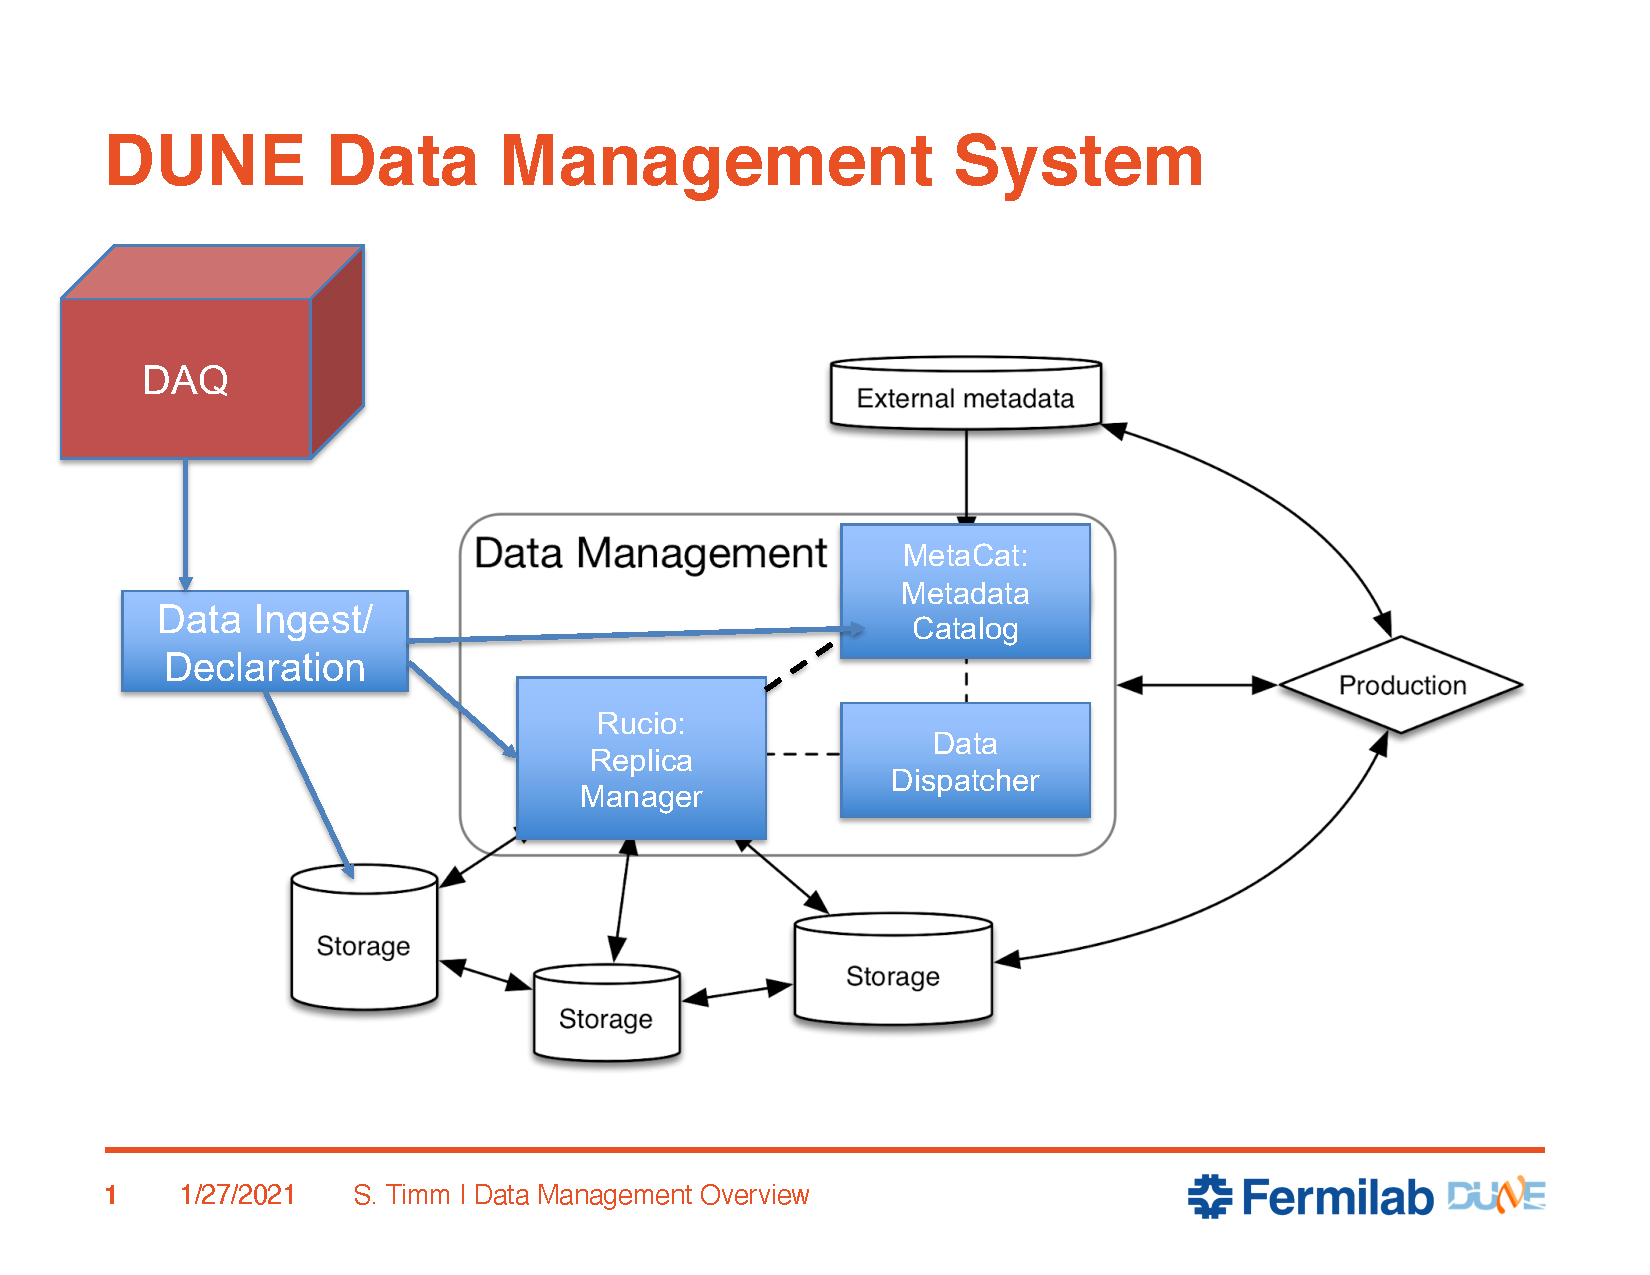
\includegraphics[height=8cm]{graphics/DataManagement/data_mgmt_diagram.pdf}
% \end{dunefigure}
% \todo{Get better figure}
\section{Future Components\hideme{Heidi added 3/9}}
We propose to replace the \dword{sam} system with %a 
the following set of components: 

\begin{itemize}
\item Metadata Catalog: stores file characteristics but not locations;    
    \item Data Ingest Manager: takes in data from detector sites, declares it to the catalog and transfers to the managed storage system;
    \item R\dword{rucio}-based Replica Manager: stores the physical location of files and provides tools to move them between storage elements; and
    \item Data Dispatcher: interacts with user and production processing systems%.  It provides 
    to provide file location information from the Replica Manager to clients and can track file processing. 
\end{itemize}

The \dword{rucio} system is already being used for file movement.  We are testing use of \dword{metacat}/\dword{rucio} in hopes of putting them into production for \dword{pdsp2} runs late in 2022. 


\section{Metadata Catalog \hideme{updated 3/9 may still be too long}}

The current \dword{sam} data catalog combines file description with location and delivery.  The new \dword{metacat} catalog will provide the permanent file description information, with location and delivery handled by \dword{rucio} and a data dispatch system. 
A prototype version of \dword{metacat} has been produced and is described in Reference~\cite{Mandrichenko:2021spd}. 

DUNE file metadata includes mandatory and optional fields and can be represented to the API by a Python dictionary or a \dword{json} file. 
As with \dword{sam}, the metadata includes a description of the file itself and data about how it was created, including enough information to follow the full processing chain.   



%\hideme{put in a metacat listing for the file above. }
% \begin{verbatim}                   {
%  "file_name": "np04_raw_run005141_0006_dl1_reco1_42477998_0_20210324T231631Z.root",
%  "file_id": 52593202,
%  "create_date": "2021-03-25T16:01:37+00:00",
%  "user": "dunepro",
%  "update_date": "2021-03-25T17:03:05+00:00",
%  "update_user": "dunepro",
%  "file_size": 3599190934,
%  "checksum": ["enstore:3896981774"],
%  "content_status": "good",
%  "file_type": "detector",
%  "file_format": "artroot",
%  "data_tier": "full-reconstructed",
%  "application": {"family": "art", "name": "reco","version": "v09_09_01"},
%  "process_id": 15298375,
%  "event_count": 107,
%  "start_time": "2021-03-24T23:27:22+00:00",
%  "end_time": "2021-03-25T15:59:16+00:00",
%  "data_stream": "physics",
%  "beam.momentum": 7.0,
%  "detector.hv_value": 180,
%  "DUNE.campaign": "PDSPProd4",
%  "DUNE_data.acCouple": 0,
%  "DUNE_data.calibpulsemode": 0,
%  "DUNE_data.DAQConfigName": "np04_WibsReal_Ssps_BeamTrig_00021",
%  "DUNE_data.febaselineHigh": 2,
%  "DUNE_data.fegain": 2,
%  "DUNE_data.feleak10x": 0,
%  "DUNE_data.feleakHigh": 1,
%  "DUNE_data.feshapingtime": 2,
%  "DUNE_data.inconsistent_hw_config": 0,
%  "DUNE_data.is_fake_data": 0,
%  "runs": [[5141,1,"protodune-sp"]],
%  "parents": [{
%   "file_name": "np04_raw_run005141_0006_dl1.root", "file_id": 6606706}]
% }
 
The DUNE data  management system operates on a collection of ``physical'' copies of files (or objects), moving them between storage elements and making them available to the data processing and analysis. 
A single  ``logical'' file can have multiple ``physical'' replicas across multiple storage elements. The \dword{metacat} package replaces the \dword{sam} file description function and generalizes it to objects.  
\dword{metacat} stores metadata about logical files and objects and makes it possible to select ``interesting'' logical files based on criteria expressed in terms of metadata parameters. 

The \dword{metacat} design builds on \dword{sam} experience, preserving the useful concepts while introducing additional flexibility and constraints where needed.   For example:

\begin{itemize}  
\item To enforce reproducibility, %anne free-form datasets no longer exist and must be explicitly modified. 
datasets no longer exist as free-form and must be explicitly modified.
\item Metadata values are more flexible.
\item Namespaces are introduced to separate different functions (e.g., user %and
versus production files)
\item External databases (e.g., for run information) are used where needed.  In \dword{sam}, run characteristics were often duplicated in every associated file.
\item Modification permissions are more granular.
\end{itemize} 

%anne need at least two subsections in a section (or none) \subsection{MetaCat Project Objectives, Scope and Requirements}
Although the main target user of the project is \dword{protodune}/DUNE, \dword{metacat} is supposed to be generic enough to be usable by %multiple 
other experiments, as well.   \dword{metacat} has to satisfy the following general requirements: 

\begin{itemize} 
\item 
The Metadata representation must be powerful, flexible and abstract enough to accommodate a wide range of metadata data types and possibly complex metadata structures. 

\item
It needs to scale to at least 100 million objects and likely into the tens of billions of objects. %Kirby - rough guess based on NOvA and MicroBooNE experience and 20 years of DUNE operations \todo{(anne) 100M OR beyond? How far beyond? This is ambiguous}

\item
The unit of operation of the catalog should be an abstract ``file'' or ``object'' with a  minimal but sufficient set of predefined   attributes and the ability to add user-defined   attributes in a flexible and convenient way. 

\item 
The file selection mechanism must be powerful and at the same time simple enough to be able to express a wide range of metadata selection criteria. 

\item 
The \dword{metacat} should not need knowledge of physical file replicas, aside from a checking mechanism to make certain that all physical objects have logical representations in the catalog. 

\end{itemize} 
 

Based on our experience with \dword{sam}, an important improvement is to provide a mechanism to use data from external metadata sources, such as conditions or runs databases, as part of metadata queries without copying the external data into or making it appear as part of the metadata database. 

\section{Metacat Data Model \hideme{Updated 3/9}}
In \dword{sam}, files were identified by a unique immutable name within a single namespace.  To support  multiple use cases (for example user and production spaces) \dword{metacat}'s objects %and 
can be identified  by names within namespaces. The name of an object is unique within its namespace. A namespace/name pair uniquely identifies  an object in \dword{metacat}. In addition to namespace/name, files are assigned unique text identifiers. These identifiers are primarily for internal use within the \dword{metacat} database, but are available to the user. At the time of the file declaration, the user can specify a file ID, which must be unique, otherwise \dword{metacat} will generate a unique file ID. After a file is declared to \dword{metacat} it can be renamed. Both namespace and name can be changed, provided the new namespace/name pair is unique. However, file ID can not be changed. 

As in \dword{sam}, \dword{metacat} stores metadata associated with files and datasets. %HMS tried to clean up this definition.  Made a new glossary term
A \dword{metacatdataset} is a collection of files. A \dword{metacatdataset} can have child \dword{metacatdataset}.  %A dataset can be set to be ``monotonic,'' which means files can not be added to or removed from the dataset. %HMS 3/9, or be frozen. %anne  - files cannot be added or removed from the dataset. 
Unlike the active \dwords{samdataset} defined   in \dword{sam}, files must be explicitly added to and removed from a \dword{metacatdataset}. 
%\todo{(anne) a nonmonotonic dataset?}
A file can belong to zero or more \dword{metacatdataset}. \hideme{HMS - I think this may confuse the reviewers suggest leaving it out There is no requirement that the file namespace  be related in any way to the namespace(s) of the \dword{metacatdataset}(s) the file belongs to. If a file belongs to a child \dword{metacatdataset}, it does not %anne mean it belongs HMS I like the necessarily 
necessarily belong to its parent \dword{metacatdataset}. However, the query language discussed below allows recursive inclusion of files from child \dword{metacatdataset} into query results.}


As in \dword{sam} there can be a many-to-many provenance relationship between files. A file can have zero or more derived (child) files and zero or more parent files. The system makes sure the provenance relationship is not circular. 
Metadata attributes are name-value pairs. Any file or \dword{metacatdataset} can have zero or more metadata attributes. Attribute names are alphanumeric words optionally combined with dots. Any \dword{json} structure can be an attribute value. Therefore, a file or a \dword{metacatdataset} attribute set is a \dword{json} dictionary. 

Here is an example with the same file described in \dword{sam} above. Note the nine fixed fields at the top followed by freer-form metadata. 

\begin{verbatim}
checksums      :    {'md5': 'ea8d1a009f23accf9582f9e2bd7f58fd', 'adler32': 'c689390f', 'enstore': '3896981774'}
children       :    ['52593351']
created_timestamp:  1616688097.41347
creator        :    dunepro
fid            :    52593202
name           :    np04_raw_run005141_0006_dl1_reco1_
            42477998_0_20210324T231631Z.root
namespace      :    pdsp_det_reco
parents        :    ['6606706']
size           :    3599190934
metadata       :   {
    'DUNE.campaign': 'PDSPProd4',
    'DUNE_data.DAQConfigName',
    'np04_WibsReal_Ssps_BeamTrig_00021',
    'DUNE_data.acCouple': 0,
    'DUNE_data.calibpulsemode': 0,
    'DUNE_data.detector_config':  ...... 
    'DUNE_data.detector_config.object': ['cob2_rce01', 'cob2_rce02',
    'DUNE_data.feshapingtime': 2,
    'DUNE_data.inconsistent_hw_config': 0,
    'DUNE_data.is_fake_data': 0,
    'beam.momentum': 7,
    'data_quality.online_good_run_list': 1,
    'detector.hv_value': 180,
    ...... many other items not shown  .....
}


 \end{verbatim}

\subsection{Ownership and Permissions }

A \dword{metacat} user  is identified  by a unique username. A user can be a member of zero or more roles (groups). Namespaces and attribute categories have owners. A namespace or category owner can be either an individual user or a role. If the namespace or the category is owned by the role, %HMS OK anne it means 
that means it is automatically owned by all role members. 
The namespace owner automatically owns all the datasets and files in that namespace (either directly or via the role membership). Ownership does not automatically propagate along the dataset parent/child or file provenance relationships. 
Only the owner of the dataset and file %anne owner 
can add or remove files from the dataset. Only the owner of the dataset can change their metadata attributes. The same is true for files in that only the owner of a file can change their metadata attricutes. %Kirby - clarified. Hopefully it's correct. \todo{(anne) the `and' and 'or' are significant here?}

\subsection{Queries} 
One of the most important parts of the \dword{metacat} functionality is the ability to query the database for ``interesting'' files. Essentially, the query is a logical expression in terms of file and/or dataset metadata attributes, file provenance relationship, and dataset parent/child relationship. There are two types of queries in \dword{metacat}-file queries and dataset queries. File queries return a set of files (a list of file IDs) whereas dataset queries return a list of datasets. The file and dataset lists are not guaranteed to have a consistent order, so they are in fact ``sets'' rather than ``lists.'' 
A query is merely a formula specifying the selection criteria. \dword{metacat} never saves the results of the query, so re-running a query can produce different results as files are  added/removed from the system, to/from the datasets or their metadata attributes change.
%HMS took Anne's suggestion added/removed to/from the datasets or their %metadata attributes change. 
However, there is an option to save results of the file query as a new \dword{metacatdataset} or add selected files to an existing \dword{metacatdataset}. 
A query can be saved into the database under a name within a namespace. This function can be used to publish complicated queries and make them reusable by other users. 

\subsection{MetaCat Query Language (MQL)}
The original \dword{sam} query language was produced in the late 1990s to provide a restricted command set and  avoid having users execute full SQL queries.

In \dword{metacat}  the query is written in a specialized query language, \dword{mql}. \dword{mql} allows the user to specify file/dataset metadata attribute criteria, use \dword{metacatdataset} parent/child relationships and file provenance relationships to select a set of file or a \dword{metacatdataset}. Further, simple queries can be combined into more complicated ones using logical operations like union, join, subtraction. Named queries can be referred to from within the \dword{mql} expression by their name. 

\subsection{External data sources }
\dword{metacat}   functionality includes the ability to access external metadata sources, such as conditions databases, and use the data stored there to filter file selection results. In order to make an external metadata source available to \dword{metacat} instance,  a Python plug-in module with a standard interface must be provided.  Once the module is plugged into a \dword{metacat} instance, it can be referred to in the \dword{mql} query as a named filter  and used to filter results of an intermediate query or queries within the \dword{mql} expression or even ``inject'' metadata from the external source into the query and make it available as a  selection criterion. 

\subsection{Architecture and Interfaces}
\dword{metacat} is a typical web services database application. The underlying database is not exposed to end users. It can be accessed via a Python API, but the primary method of interacting with the system is through a web service or web GUI. Use of this REST-based web service 
%Kirby - standard type of API interface. \todo{(anne) what's REST?}
improves the scalability and cacheability of the system and completely unties the server side from the client implementation. Any standard HTTP/HTTPS client can interact with the system either directly or through a standard HTTP proxy or cache. 


The system publishes the following interfaces: 
\begin{itemize} 
\item Direct database access Python API, 

\item Web services REST interface, 

\item Python client side API that communicates with the server via HTTP, and 

\item 
Command line interface with a basic set of commands to enter (modify) data into the database and to query the database. 
\end{itemize}


\subsection{Current Status} 
\dword{metacat} is currently in the testing phase in parallel with the \dword{sam} catalog.  A plan for switching from \dword{sam}/\dword{rucio} is being finalized with full deployment either during \dword{pdsp2} or for subsequent processing steps in 2022-2023. 


%     \end{verbatim}

\section{Data Ingest Manager \hideme{HMS moved here 3/9}}

The Data Ingest Manager will run at detector sites.  It consists of two components:  the Ingest Daemon and the Declaration Daemon.  The Ingest Daemon will 
run at each detector location, at CERN EHN1, SURF surface and Fermilab. Each instance will
%\todo{HMS (anne) pls clarify how this interacts with the portion of the DAQ that is situated right outside the detector. And is this ND or FD? And if FD, right outside each module? }
detect new files in the data store, extract the metadata and add new metadata fields
if necessary, calculate the checksum of the files, initiate and monitor the transfers to the first managed 
storage element, and send a signal back to the \dword{daq} when the file has been transferred and can be deleted from the data store.
Files will be transferred to a drop box on the nearest managed storage element, using \dword{fts3} %Kirby - done. \todo{add a note about FTS3 to the glossary}
as the transport mechanism.  

The Declaration Daemon will run on or near a storage element that is managed by the replica manager. %Kirby - yes, I think that transfer failures should stay within the Ingest Daemon and FTS3. \todo{Is it safe to declare after transfer? this means transfer failures can't be tracked using the \dword{metacat} }
It will detect new files that have been added to the drop box, and declare them to the metadata catalog and the replica manager.  It will then instruct the replica manager to send these files to permanent tape-backed storage and monitor the transfer to be sure that this has been done, and then send a signal to remove them from the temporary drop box.

These daemons will be performing most of the functions that the current data transport system does, they only 
require modification to contact the new replica manager and metadata catalog rather than the current ones.  The 
requirements for these daemons have been defined   and %anne we expect 
coding work is expected to start in mid to late summer 2021. 
\todo{(anne) Update please! Did it start?}

\section{Rucio Replica Manager \hideme{HMS updated 3/9}}

The replica manager must track the physical location of  data files %where all data files are located 
and ensures that they 
are moved from point to point as needed. The choice  that we have made 
for this functionality is the \dword{rucio} data
management system~\cite{Baritsis:2019csbs}.  This system was originally developed by the ATLAS experiment and has now been deployed to 
a number of other HEP and astronomy experiments.  DUNE has had a \dword{rucio} server since 2019.  All raw data that was
taken in the fall 2018 \dword{pdsp} (\dword{np04}) run and since that time, as well as all raw data taken by the \dword{pddp} (\dword{np02}) run, is tracked by \dword{rucio}.  All output of \dword{mc} simulation and reconstruction also is tracked by \dword{rucio}. \dword{dune} plans to take full advantage of the data lifetime features of \dword{rucio}.

\dword{rucio} is a rule-based system.  Files are sent to remote servers via a system of rules
that are created by the experiment data managers. \dword{rucio} provides tools to implement those rules.   Data can be accessed interactively or in batch jobs and
\dword{rucio} has a built-in system of delivering the URI of the closest replica to the running job for access via streaming.

The main work that remains to be done in implementing the \dword{rucio} server is  back-loading all relevant 
data from the legacy \dword{sam} system into \dword{rucio}.  Currently about 50\% of the data by volume is known by \dword{rucio} but only about 25\% of the files by file count are declared to it. 

DUNE has contributed several features to the \dword{rucio} base software.  These include a new method to map from the \texttt{scope:filename} logical file name to the path-based directory structure that we use on tape sites.  

We also have added a hook that requires any new files declared to \dword{rucio} to be also declared to the \dword{metacat} system.  We have modularized the \dword{vo} customization code, and we have made the command line client lighter-weight with fewer external dependencies and fewer conflicts with other Python software. 

\dword{rucio} has a internal metadata functionality but our evaluation indicates that it doesn't provide the full functionality required by DUNE physics and offline processing,%currently provided by the \dword{sam} catalog,
and thus DUNE has proceeded to develop its own metadata catalog. 

\section{Data Dispatcher \hideme{HMS 3/9 updated}}

The \dword{datadis} replaces the project management and file delivery functions that were previously done by the \dword{sam} system.  The \dword{datadis} functions include:
\begin{itemize}
    \item Creating projects to process collections of data,
    
    \item Delivering file handles of the files to consumers,
    
    \item Keeping track of the project progress, including consumer status and files consumed,
    
    \item Keeping record of projects, consumers, and file consumption for a specified amount of time,
    
    \item Providing project monitoring and control to a user or a client, and
    
    \item Organizing and coordinating data processing among data consumer processes.

\end{itemize}

Work has begun on a prototype \dword{datadis} which re-uses existing \dword{sam} code where appropriate.  The exact boundary between the \dword{datadis} and the Workflow System (see Chapter \ref{ch:wkflow}) has not been finalized but it is likely that other \dword{fnal} experiments will need the \dword{datadis} functionality if \dword{sam} is deprecated. 



\section{Tools \hideme{Timm - needs more}}

The data management system relies on several sets of underlying tools.  The \dword{rucio} replica manager is dependent on the CERN File Transfer Service (FTS3)~\cite{Kiryanov:2015fts} to actually move files from one storage element to another, although it can also use the proprietary
Globus protocol 
\todo{(anne) add Globus to gloss - and GFAL2 (and FTS3 as noted earlier}
particularly when moving files to and from US \dword{hpc} centers.  The FTS3 service in turn is dependent on the
GFAL2 (Grid File Access Library) set of utilities.





\end{document}